% =====================================================================
%  第三部分  代码逐行解释
% =====================================================================
\part{代码逐行解释}

前两部分讲清了原理。这一部分把原理和代码对应起来，
逐段说明每一行在做什么，以及为什么必须这么写。

阅读这一部分之前，建议先打开代码文件对照着看。

% =====================================================================
\section{代码总览}

\subsection{文件分工}

整套代码分成两类。一类是求解器，负责算出结果；
另一类是驱动脚本，负责调用求解器、输出表格和图。

\begin{center}
\begin{tabular}{@{}llp{7.4cm}@{}}
\toprule
文件 & 类型 & 职责 \\
\midrule
\texttt{common.py} & 基础 & 存放全部参数、物性公式、附件读取、环境标定 \\
\texttt{spectral.py} & 求解器 & 主求解器，实现第二部分讲的全部方法 \\
\texttt{analytic\_p1.py} & 求解器 & 问题一的闭式解，用来验证主求解器 \\
\texttt{fv\_theta.py} & 求解器 & 对照格式一：节点中心有限体积加定步长 $\theta$ 法（Crank--Nicolson，前 4 步用 $\theta=1$ 做 Rannacher 启动，物性冻结在上一时间步） \\
\texttt{fv\_uniform.py} & 求解器 & 对照格式二：守恒型有限体积加等步长后向欧拉加 Picard 迭代（迭代 3 次） \\
\texttt{run\_all.py} & 驱动 & 一键跑出全部结果与验证 \\
\texttt{make\_results.py} & 驱动 & 生成四个结果文件 \\
\texttt{make\_figs.py} & 驱动 & 生成剖面与干燥曲线插图 \\
\texttt{make\_fig3.py} & 驱动 & 生成收敛性插图 \\
\texttt{sensitivity.py} & 驱动 & 参数扰动灵敏度分析 \\
\texttt{env\_compare.py} & 驱动 & 烘房环境两种口径对比 \\
\texttt{figs.py} & 驱动 & 生成本文档的七张教学插图 \\
\bottomrule
\end{tabular}
\end{center}

两套对照格式都用均匀网格加有限体积，共同点是局部守恒、离散矩阵三对角。
区别在时间推进与物性处理这两处。
对照格式一是节点中心有限体积配定步长的 $\theta$ 法：
取 $\theta=\dfrac{1}{2}$ 就是 Crank--Nicolson，时间上二阶精度；
前 4 步改用 $\theta=1$，也就是后向欧拉，这叫 Rannacher 启动，
目的是压掉初值不光滑引起的振荡；
物性在整个时间步内冻结在上一时间步的值上，不再更新。
对照格式二是守恒型有限体积配等步长后向欧拉，时间上一阶精度；
非线性物性用 Picard 迭代处理，每个时间步里把物性按新解重算并重新组装，
一共迭代 3 次。这样两套格式除了都用均匀网格和有限体积之外，
离散族、时间格式、非线性处理全都不同。

\why{为什么要写三个求解器}
因为要判断结果对不对。一个程序跑出来的数字，
如果自己写错了公式，它也不会报错，只会给出一个看起来正常的错数。
唯一的办法是用另一种完全不同的方法算同一个问题，
如果两者结果一致，那么同时写错的可能性就很小。
这叫做交叉验证。

\subsection{为什么把参数单独放一个文件}

如果每个脚本里都写一遍参数数值，改一个数就要改很多地方，
很容易漏改，导致不同脚本用的参数不一样，结果对不上。
把所有参数集中在 \texttt{common.py} 里，
其他脚本都从这里取，就避免了这个问题。

\keypoint
代码组织的原则是：参数集中存放，求解器与驱动分离，关键结果用多个独立方法验证。

% =====================================================================
\section{主求解器 spectral.py 逐段解释}

\subsection{文件头部与导入}

\begin{lstlisting}[language=Python]
# -*- coding: utf-8 -*-
"""主求解器：坐标 u=(r/R)^2 下的 Chebyshev 谱配置 + 自适应隐式时间积分。

方法要点：
  * 坐标：取 u=(r/R)^2 为自变量
  ...（docstring 的其余各行在这里省略，内容见下文）
"""
import numpy as np
from scipy.integrate import solve_ivp
import common as cm
\end{lstlisting}

这个文件的前 18 行分成三段。第 1 行是编码声明，
第 2 到 15 行是模块的 docstring，
第 16 到 18 行是三个 import 语句。

第一行是编码声明，告诉 Python 这个文件用 UTF-8 编码，
这样文件里的中文注释才不会乱码。

第 2 到 15 行是 docstring，一共 14 行。
docstring 是 Python 里写在文件开头或者函数开头的一段说明文字，
外层用三个连续的双引号字符括起来。
它在程序运行时只是一段字符串，不参与任何计算，
但可以用 help 命令打印出来，也可以被文档工具自动收集。
这个 docstring 写的是本文件的方法要点，一共四条。

\begin{itemize}[leftmargin=1.8em,itemsep=2pt]
\item 坐标：取 $u=(r/R)^2$ 为自变量，
  使圆柱的拉普拉斯算子在 $u=0$ 处完全正则，不含 $1/u$ 的奇异项，
  轴心与表面都不需要任何特殊的控制体处理。
  这是本方法与常规 $r$ 坐标离散最核心的差别。
\item 空间：切比雪夫--高斯--洛巴托谱配置，谱精度、全局耦合；
  解在 $u$ 上解析，所以谱收敛成立。
\item 时间：自适应变阶隐式 BDF（即 scipy 的 \texttt{solve\_ivp}），
  物性在每个右端项求值处重新计算，误差由 rtol 与 atol 直接控制；
  另外提供 Radau 与 LSODA 供交叉验证。
\item 边界：以通量形式配置。
  内部节点的通量由谱微分给出，
  表面节点的通量直接取 Robin 条件的物理值，
  因此边界条件以物理通量的身份精确进入离散方程。
\end{itemize}

第 16 行导入 numpy。numpy 是 Python 的科学计算库，
它提供了数组这种数据结构。数组和普通列表的区别是：
数组支持整体的加减乘除，不需要写循环。

举例说明这个区别。如果要把十个数的每个都乘以二，
用列表要写

\begin{lstlisting}[language=Python]
result = []
for v in my_list:
    result.append(v * 2)
\end{lstlisting}

用数组只要写

\begin{lstlisting}[language=Python]
result = my_array * 2
\end{lstlisting}

代码短很多，运行也快很多。本题里到处都要对整条半径上的量做运算，
用数组是必须的。

第 17 行导入 scipy 的求解器 \texttt{solve\_ivp}。
它负责解法 \eqref{eq:semi} 那样的常微分方程组，
也就是说，第二部分第七章讲的自适应变阶 BDF 方法，
我们不需要自己写，直接调用它。

第 18 行导入我们自己写的 \texttt{common.py}，并给它起个别名 \texttt{cm}。
这样后面写 \texttt{cm.R0} 就能取到半径这个参数。

\subsection{函数 cheb\_matrices：构造微分矩阵}

\begin{lstlisting}[language=Python]
def cheb_matrices(N):
    x = np.cos(np.pi * np.arange(N + 1) / N)
    c = np.hstack([2.0, np.ones(N - 1), 2.0]) * ((-1.0) ** np.arange(N + 1))
    X = np.tile(x, (N + 1, 1)).T
    dX = X - X.T
    D = np.outer(c, 1.0 / c) / (dX + np.eye(N + 1))
    D -= np.diag(D.sum(axis=1))
    return D, D @ D, x
\end{lstlisting}

这个函数实现第二部分第六章里的式 \eqref{eq:chebnode}、
式 \eqref{eq:dij} 和式 \eqref{eq:dii}。逐行说明。

第一行

\begin{lstlisting}[language=Python]
x = np.cos(np.pi * np.arange(N + 1) / N)
\end{lstlisting}

\texttt{np.arange(N+1)} 生成数组 $[0,1,2,\dots,N]$。
乘以 $\pi$ 再除以 $N$，得到 $[0,\pi/N,2\pi/N,\dots,\pi]$。
最后取余弦，得到 $x_j=\cos(j\pi/N)$，
这正是式 \eqref{eq:chebnode} 的定义。

注意这个数组是从 $1$ 递减到 $-1$ 的，
因为 $\cos0=1$，$\cos\pi=-1$。

第二行

\begin{lstlisting}[language=Python]
c = np.hstack([2.0, np.ones(N - 1), 2.0]) * ((-1.0) ** np.arange(N + 1))
\end{lstlisting}

\texttt{np.ones(N-1)} 生成 $N-1$ 个 $1$。
\texttt{np.hstack} 把三部分横向拼起来，得到
$[2,1,1,\dots,1,2]$，长度是 $N+1$。
这对应式 \eqref{eq:dij} 里定义的 $c_0=c_N=2$，中间的都是 $1$。

后面乘上 $(-1)^j$，得到带符号的系数，记作 $c_j$。
这样做的目的是把式 \eqref{eq:dij} 分子上的 $(-1)^{i+j}$ 收进系数 $c$ 里：
$c_i$ 里含 $(-1)^i$，$c_j$ 里含 $(-1)^j$，
又因为 $1/(-1)^j$ 等于 $(-1)^j$，
所以下一步算出的商 $c_i/c_j$ 正好给出 $(-1)^{i+j}$。
符号在这里一次到位，代码里不存在需要事后纠正的符号问题。

第三行

\begin{lstlisting}[language=Python]
X = np.tile(x, (N + 1, 1)).T
\end{lstlisting}

这里 $x$ 是长度为 $N+1$ 的一维数组，也就是一个列向量。
\texttt{np.tile} 把向量 $x$ 复制成 $N+1$ 行，得到一个每一行都等于 $x$ 的矩阵。
再取转置，得到的矩阵 $X$ 的每一列都等于完整的 $x$。
所以 $X$ 的第 $i$ 行的所有元素都相等，第 $i$ 行上的公共值就是 $x_i$，
写成元素形式是
\begin{equation}
X_{ij}=x_i .
\end{equation}

第四行

\begin{lstlisting}[language=Python]
dX = X - X.T
\end{lstlisting}

\texttt{X.T} 是 $X$ 的转置，$X$ 的列在转置以后变成行，
所以 \texttt{X.T} 的第 $i$ 行的所有元素都等于 $x_j$，写成元素形式是
\begin{equation}
(X^{\mathrm{T}})_{ij}=x_j .
\end{equation}
两者相减，得到 $dX$ 的第 $i$ 行第 $j$ 列等于
\begin{equation}
dX_{ij}=x_i-x_j .
\end{equation}

这正是式 \eqref{eq:dij} 分母里需要的 $x_i-x_j$，符号完全一致，
所以后面做除法时不需要任何修正。

\why{为什么这里不直接写 x\_i 减 x\_j}
因为用矩阵运算表达更简洁。用一个转置相减就得到全部两两差值，
不需要写双重循环。这是 numpy 的广播机制，
也是科学计算代码的典型写法。

第五行

\begin{lstlisting}[language=Python]
D = np.outer(c, 1.0 / c) / (dX + np.eye(N + 1))
\end{lstlisting}

\texttt{np.outer(c, 1.0/c)} 生成矩阵，第 $i$ 行第 $j$ 列等于 $c_i/c_j$。
这是式 \eqref{eq:dij} 的第一个因子。
把它按元素除以 $dX$ 加单位矩阵，就得到 $D$。
当 $i$ 不等于 $j$ 时

\begin{equation}
D_{ij}=\frac{c_i/c_j}{x_i-x_j},
\end{equation}

与式 \eqref{eq:dij} 完全一致。
也就是说，$D$ 的第 $i$ 行第 $j$ 列等于 $c_i$ 除以 $c_j$，再除以 $x_i$ 减 $x_j$。

\texttt{np.eye(N+1)} 是单位矩阵，对角线上是 $1$，其余是 $0$。
加上它是为了避免除以零，因为 $dX$ 的对角线上全是零。
加上单位矩阵以后，对角线上的分母由 $0$ 变成 $1$，
这一处的值暂时等于 $c_i/c_i$，也就是 $1$，除法不会出错。

至于对角线上的值是否因此变错，下一行会修正。

第六行

\begin{lstlisting}[language=Python]
D -= np.diag(D.sum(axis=1))
\end{lstlisting}

\texttt{D.sum(axis=1)} 把每一行的元素求和，得到一个长度 $N+1$ 的向量。
此时对角线上的值是 $1$，所以第 $i$ 行的和等于 $1$ 加上该行其余元素之和。
\texttt{np.diag} 把这个和放到一个对角矩阵的对角线上。
\texttt{D -=} 表示从 $D$ 中减去这个对角矩阵。

相减以后，对角线上的那个 $1$ 被换成该行其余元素之和的相反数，
因为
\begin{equation}
1-\left(1+\sum_{j\ne i}D_{ij}\right)=-\sum_{j\ne i}D_{ij},
\end{equation}
而不在对角线上的元素没有变动。

于是第 $i$ 行的和变成

\begin{equation}
\sum_{j\ne i}D_{ij}+\left(-\sum_{j\ne i}D_{ij}\right)=0 .
\end{equation}

这正是式 \eqref{eq:dii} 要求的行和为零。
这种写法常被说成把对角线改成负的行和，
准确地说，是改成该行其余元素之和的相反数，
也就是式 \eqref{eq:dii} 给出的对角线赋值公式。

\why{为什么不直接算出对角线再填进去}
减对角矩阵这个写法同时完成了修正和清零两件事，
一行代码解决，而且不需要把对角线元素单独挑出来处理。

第七行返回三个值：一阶微分矩阵 $D$、
二阶微分矩阵 $D^2$，也就是 $D$ 与自身相乘，以及节点坐标 $x$。

\subsection{类的初始化}

\begin{lstlisting}[language=Python]
class HerbSolver:
    def __init__(self, N, prob, shrink=False):
        self.N = N
        self.Np = N + 1
        self.prob = prob
        self.shrink = shrink
        Dx, D2x, x = cheb_matrices(N)
        self.u = (1.0 - x) / 2.0
        self.Du = -2.0 * Dx
\end{lstlisting}

类的作用是把数据和方法打包在一起。
创建对象时传入三个参数：节点数 $N$、问题编号、是否考虑收缩。

\begin{itemize}[leftmargin=1.8em,itemsep=2pt]
\item \texttt{self.N} 保存节点数。
\item \texttt{self.Np} 保存节点总数，等于 $N+1$。
  变量名后面的 \texttt{p} 表示 plus。
\item \texttt{self.prob} 保存问题编号，取 $1$、$2$、$3$ 或 $4$，
  用来决定用哪一组物性公式。
\item \texttt{self.shrink} 是逻辑值，只有问题四才设为真。
\end{itemize}

\begin{lstlisting}[language=Python]
self.u = (1.0 - x) / 2.0
\end{lstlisting}

这一行实现式 \eqref{eq:map01} 的映射，把切比雪夫节点变成 $u$ 坐标的节点。
结果满足 $u_0=0$、$u_N=1$，对应圆心和表面。

\begin{lstlisting}[language=Python]
self.Du = -2.0 * Dx
\end{lstlisting}

这一行实现式 \eqref{eq:du}。因为 $u=\dfrac{1-x}{2}$，
对 $u$ 求导等于对 $x$ 求导再乘 $-2$。

\why{为什么把微分矩阵存起来而不是每次重算}
因为它在整个求解过程中不变，算一次就够了。
存下来可以节省时间。这叫空间换时间。

\begin{figure}[H]
\centering
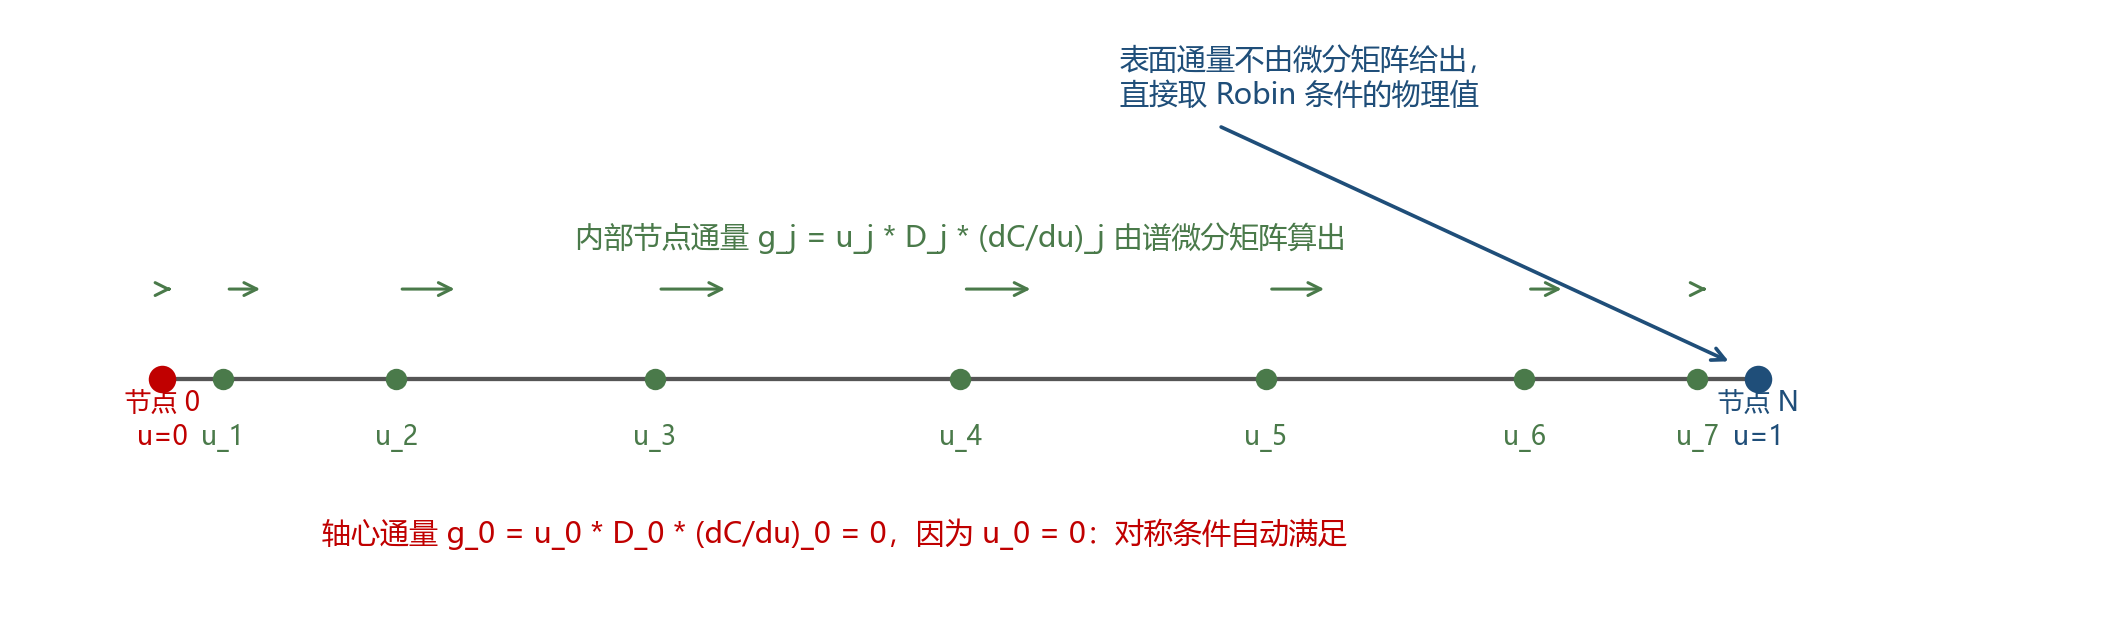
\includegraphics[width=0.96\textwidth]{fig/fig_flux.png}
\caption{通量形式的谱配置。内部节点的通量由谱微分矩阵算出，表面节点的通量直接取自 Robin 边界条件的物理值，轴心节点的通量因为 u 等于零而自动为零。}
\label{fig:flux}
\end{figure}

\subsection{右端项函数：核心中的核心}

\begin{lstlisting}[language=Python]
def rhs(self, t, y):
    N, Np = self.N, self.Np
    C = y[:Np]
    T = y[Np:]
    R = self.R_of(t)
    rho, cp, k, D = cm.props(self.prob, C, T)
\end{lstlisting}

\texttt{rhs} 是 right hand side 的缩写，意思是方程的右端。
积分器在每一步会反复调用这个函数，
传入当前时刻 $t$ 和当前状态 $y$，
要求我们返回状态的导数 $\dfrac{\mathrm{d}y}{\mathrm{d}t}$。

\texttt{y} 是一个长度 $2(N+1)$ 的数组，
前一半存含水率，后一半存温度。这样打包的原因稍后解释。

\texttt{y[:Np]} 是切片操作，取出前 $N+1$ 个元素，赋给 $C$。
\texttt{y[Np:]} 取出从下标 \texttt{Np} 开始到末尾的全部元素，赋给 $T$。
下标 \texttt{Np} 等于 $N+1$，而 Python 的下标从 $0$ 开始计数，
所以 $T$ 的第一个元素在数组里排第 $N+2$ 位。

\why{为什么把两个未知量放进同一个数组}
因为积分器只能处理一个未知向量。
把含水量和温度首尾相接拼成一个长向量，
就能用同一个积分器同时推进两个场，
而且能自动处理两者之间的耦合。

\begin{lstlisting}[language=Python]
R = self.R_of(t)
rho, cp, k, D = cm.props(self.prob, C, T)
\end{lstlisting}

第一行取当前半径。问题一到问题三里它恒等于 $R_0$，
问题四里它按附件二的数据插值得到。

第二行调用 \texttt{common.py} 里的 \texttt{props} 函数，
根据当前的含水率和温度算出四个物性。
注意它一次性返回四个值，这叫元组解包。

\why{物性为什么在每个右端项求值处重新计算}
因为物性依赖未知量 $C$ 和 $T$。
如果只在每一步开始时算一次，整个步内都当常数用，
就相当于把方程线性化了，精度会下降。
每次求值都重算，虽然麻烦一点，
但积分器在每一步内部本来就会多次调用右端项，
这样相当于做了隐式迭代，精度更高。

接下来是水分部分。

\begin{lstlisting}[language=Python]
# 水分：g = u*D*dC/du
gC = self.u * D * (self.Du @ C)
gC[N] = 0.5 * cm.hm * R * (self.C_air(t) - C[N])
dC = (4.0 / R ** 2) * (self.Du @ gC)
\end{lstlisting}

先解释通量这个概念。第二部分第五章的式 \eqref{eq:mass-u} 里，
空间部分写成

\begin{equation}
\frac{4}{R^2}\frac{\partial}{\partial u}\left(uD\frac{\partial C}{\partial u}\right).
\end{equation}

如果记

\begin{equation}
g(u) = u\,D\,\frac{\partial C}{\partial u},
\label{eq:fluxdef}
\end{equation}

那么整个空间项就是 $\dfrac{4}{R^2}\dfrac{\partial g}{\partial u}$。
这个 $g$ 叫通量，它表示单位时间通过单位截面的物质量。

把这个式子离散化，要做两件事：
第一，在每个节点上算出通量 $g$ 的值；
第二，对通量再求一次导数。

第一行 \texttt{gC = self.u * D * (self.Du @ C)} 完成第一件事。

\texttt{self.Du @ C} 表示矩阵乘向量，符号 \texttt{@} 是 Python 的矩阵乘法运算符。
这一步算出所有节点上 $\dfrac{\partial C}{\partial u}$ 的近似值。
这正是式 \eqref{eq:dmatrix} 的作用。

\texttt{self.u * D * (...)} 是两个逐元素乘法。
\texttt{self.u} 是节点坐标数组，
\texttt{D} 是各节点上的扩散系数数组。
逐元素相乘就是让第 $j$ 个节点上的 $u_j$、$D_j$ 和导数值相乘，
得到该节点的通量 $g_j$。这正是式 \eqref{eq:fluxdef}。

第二行 \texttt{gC[N] = ...} 单独修改最后一个节点，也就是表面的通量。

\why{为什么表面的通量不能直接用上面的公式算}
因为上面的公式算的是插值多项式的导数。
在表面处，物理条件式 \eqref{eq:bcu-C} 告诉我们通量必须等于

\begin{equation}
g_N = D\left.\frac{\partial C}{\partial u}\right|_{u=1}
= \frac{h_mR}{2}\left(C_{\mathrm{air}}-C_1\right).
\end{equation}

代码里写的是 \texttt{0.5 * cm.hm * R * (C\_air(t) - C[N])}，
和上式完全一致。这样写的好处是边界条件以物理量的身份精确进入离散方程，
而不是通过外推近似得到。

\why{圆心处要不要也单独处理}
不需要。因为代码里 \texttt{self.u} 的第一个元素是 $0$，
所以第一行算出来的 $g_0$ 自动等于零。
而 $g_0=0$ 正好就是对称条件的含义，正如第二部分第五章最后一节所说。

第三行 \texttt{dC = (4.0 / R ** 2) * (self.Du @ gC)} 完成第二件事。
把微分矩阵作用在通量数组上，得到 $\dfrac{\partial g}{\partial u}$ 在各节点的近似值，
再乘以式 \eqref{eq:mass-u} 里的系数 $\dfrac{4}{R^2}$，
得到含水率的时间导数。

\texttt{R ** 2} 是 Python 的幂运算，表示 $R^2$。

温度部分完全类似。

\begin{lstlisting}[language=Python]
# 温度：g = u*k*dT/du
gT = self.u * k * (self.Du @ T)
gT[N] = 0.5 * cm.h * R * (self.T_air(t) - T[N])
dT = (4.0 / (R ** 2 * rho * cp)) * (self.Du @ gT)
\end{lstlisting}

对应式 \eqref{eq:energy-u}。唯一的区别是左边要除以 $\rho c_p$，
因为传热方程左边是 $\rho c_p\dfrac{\partial T}{\partial t}$，
移项以后变成 $\dfrac{\partial T}{\partial t}$ 等于右端除以 $\rho c_p$。

表面条件用的是式 \eqref{eq:bcu-T}，
代码里写成 \texttt{0.5 * cm.h * R * (T\_air(t) - T[N])}，
和式 \eqref{eq:bcu-T} 完全一致。

最后打包返回。

\begin{lstlisting}[language=Python]
out = np.empty_like(y)
out[:Np] = dC
out[Np:] = dT
return out
\end{lstlisting}

\texttt{np.empty\_like(y)} 创建一个和 $y$ 同样形状的空数组。
然后把含水率的导数和温度的导数分别填进前后两半，返回。

\why{为什么要先创建空数组再填}
直接拼接两个数组也可以，但那样会多分配一次内存。
对于要在积分过程中被调用成千上万次的函数，
减少一次内存分配能明显提高速度。

\subsection{初值与求解}

\begin{lstlisting}[language=Python]
def y0(self):
    return np.concatenate([np.full(self.Np, cm.C0), np.full(self.Np, cm.T0)])
\end{lstlisting}

初值就是式 \eqref{eq:ic}。\texttt{np.full(Np, C0)} 生成 $N+1$ 个 $C_0$。
\texttt{np.concatenate} 把两个数组首尾拼接，和 \texttt{rhs} 里的拆分方式对应。

\begin{lstlisting}[language=Python]
def solve(self, t_end, t_eval=None, rtol=1e-10, atol=1e-13, method="BDF",
          events=None, max_step=np.inf, first_step=None, dense=False):
    return solve_ivp(self.rhs, (0.0, t_end), self.y0(), method=method,
                     rtol=rtol, atol=atol, t_eval=t_eval, events=events,
                     max_step=max_step, first_step=first_step, dense_output=dense)
\end{lstlisting}

这个函数是对 \texttt{solve\_ivp} 的包装。各个参数的含义是

\begin{itemize}[leftmargin=1.8em,itemsep=2pt]
\item 第一个参数 \texttt{self.rhs} 是右端函数，也就是上一小节那个。
\item 第二个参数 \texttt{(0.0, t\_end)} 是时间区间。
\item 第三个参数 \texttt{self.y0()} 是初值。
\item \texttt{method} 指定积分方法，默认用 BDF。
  也可以改成 Radau 或 LSODA 做交叉验证。
\item \texttt{rtol} 和 \texttt{atol} 是相对和绝对容差，用来控制精度。
\item \texttt{t\_eval} 指定希望输出结果的时刻，
  不指定的话积分器自己决定在哪些时刻输出。
\item \texttt{events} 用来指定事件函数，烘干时间的判定就靠它。
\end{itemize}

\why{为什么要写一层包装而不是直接调用}
因为可以把常用的默认值固定下来，
调用时只写关心的参数。而且以后要换求解器，
只要改这一个函数，其他代码不用动。

\subsection{重心插值}

\begin{lstlisting}[language=Python]
def _bary_weights(self):
    N = self.N
    w = (-1.0) ** np.arange(N + 1)
    w[0] *= 0.5
    w[N] *= 0.5
    return w
\end{lstlisting}

这个函数计算重心插值的权重。式子是

\begin{equation}
w_j = (-1)^j\times
\begin{cases}
\dfrac{1}{2}, & j=0\ \text{或}\ j=N,\\[4pt]
1, & \text{其他}.
\end{cases}
\end{equation}

代码先算出 $(-1)^j$，再把首尾两个元素各自乘 $\dfrac{1}{2}$。

首尾两个系数为什么要取 $\dfrac{1}{2}$，理由是：
切比雪夫--高斯--洛巴托节点包含两个端点，
而端点在插值公式里只贡献半个权，
所以首尾两个系数各乘 $\dfrac{1}{2}$，
其余节点不带这个因子，系数就是正负一交替。

\why{为什么需要重心插值}
因为我们要知道的不是节点上的值，
而是某些指定位置上的值。比如表格要求给出
到中心距离 $0.5$、$1.0$ 厘米处的含水率，
这些位置不一定正好落在节点上。
重心插值能在任意位置给出高精度的插值结果。

\why{为什么不用普通的拉格朗日插值公式}
因为式 \eqref{eq:basis} 那个分子分母连乘的公式在节点数多的时候
会发生严重的舍入误差，甚至上溢或下溢。
重心形式的数学结果和它完全相同，但数值上稳定得多，
计算量也小得多。这是一个已经被广泛采用的改进形式。

\begin{lstlisting}[language=Python]
def _bary(self, f, u_t):
    u_t = np.atleast_1d(np.asarray(u_t, dtype=float))
    w = self._bary_weights()
    u = self.u
    out = np.empty(u_t.shape, dtype=float)
    for k, ut in enumerate(u_t):
        diff = ut - u
        hit = np.where(np.abs(diff) < 1e-15)[0]
        if hit.size:
            out[k] = f[hit[0]]
            continue
        out[k] = np.sum(w * f / diff) / np.sum(w / diff)
    return out
\end{lstlisting}

第一行把输入统一转成数组。\texttt{np.atleast\_1d} 保证即使传进来一个数，
也会被包成长度为一的数组，这样后面的处理逻辑统一。

\texttt{np.asarray(..., dtype=float)} 保证元素是浮点数。

然后是循环，对每个目标位置 \texttt{ut} 逐个处理。

\texttt{diff = ut - u} 算出目标位置与全部节点的距离。

\texttt{np.where(np.abs(diff) < 1e-15)} 找出距离接近零的节点。
如果目标位置正好落在某个节点上，直接用该节点的值，
避免后面除以零。

否则执行最后一行，按重心公式计算

\begin{equation}
C(u_*) = \frac{\sum_j \dfrac{w_j}{u_*-u_j}C_j}{\sum_j \dfrac{w_j}{u_*-u_j}} .
\end{equation}

代码里的 \texttt{np.sum(w * f / diff)} 对应分子，
\texttt{np.sum(w / diff)} 对应分母。

\why{这个公式为什么看起来和拉格朗日公式不一样}
把式 \eqref{eq:basis} 的基函数做代数变形，
分母的连乘可以提出去作为公因子，
分子分母的公因子相消以后就剩下这个简洁的形式。
数学上两者完全等价，但重心形式每个目标点只需要两次求和，
而不是 $N$ 次连乘。

\keypoint
主求解器的结构是：一个函数构造微分矩阵，
一个类把节点、矩阵、物性、右端项打包起来，
右端项里用通量形式实现两个方程，
最后用一个包装函数调用现成的积分器。

% =====================================================================
\section{参数文件 common.py 逐段解释}

\subsection{文件定位：让程序可以搬动}

\begin{lstlisting}[language=Python]
_HERE = os.path.dirname(os.path.abspath(__file__))
_CANDIDATES = [
    os.path.join(_HERE, "..", "题目"),
    os.path.join(_HERE, ".."),
    os.path.join(_HERE, "..", ".."),
    _HERE,
]

def _find_attach(name):
    for base in _CANDIDATES:
        p = os.path.abspath(os.path.join(base, "附件", name))
        if os.path.isfile(p):
            return p
    raise FileNotFoundError(...)
\end{lstlisting}

这段代码解决的问题是：附件文件在哪个目录。

\why{为什么不直接写死附件路径}
如果写死一个绝对路径，比如从某台电脑的桌面开始的完整路径，
那么把整个文件夹复制到别的地方以后，程序就找不到附件了。
用相对位置去搜索，程序就能跟着文件夹一起搬动。

\texttt{\_\_file\_\_} 是 Python 的一个内置变量，
表示当前这个文件自己的路径。\texttt{os.path.abspath} 把它变成绝对路径，
\texttt{os.path.dirname} 取出所在目录。

\texttt{os.path.join(\_HERE, "..", "题目")} 表示从当前目录往上退一级，
再进入题目目录。\texttt{..} 在路径里的含义就是上一级。

函数逐个尝试候选位置，找到就返回，都找不到才报错。

\subsection{烘房环境的标定}

\begin{lstlisting}[language=Python]
(Tset_fit, tauT_fit), _ = curve_fit(_fT, _t_env, _Ta_env, p0=[50.2, 1800.0])
(Cset_fit, tauC_fit), _ = curve_fit(_fC, _t_env, _Ca_env, p0=[0.0509, 2800.0])

# 标定参数的报告精度：把拟合值按其有效位数保留
Tset = 50.212
tauT = 1877.5
Cset = 0.050908
tauC = 2776.3
\end{lstlisting}

上面这段是 \texttt{common.py} 的第 67 到 76 行，
其中第 70 到 72 行的注释压缩成一行印出。

\texttt{curve\_fit} 是 scipy 提供的最小二乘拟合函数，
实现的就是第一部分第三章讲的 Levenberg--Marquardt 算法。
它返回两样东西：第一样是拟合出来的参数，
第二样是参数的协方差矩阵。
左边写成 \texttt{(Tset\_fit, tauT\_fit), \_ =}，
就是把参数接出来，把协方差用下划线忽略掉。

参数的含义是：第一个是模型函数，
第二个是自变量的数据，第三个是因变量的数据，
第四个是参数的初始猜测值。

拟合的结果保存在 \texttt{Tset\_fit} 与 \texttt{tauT\_fit} 里。
随后第 70 到 76 行把实际使用的常数直接写出来：
\texttt{Tset = 50.212}、\texttt{tauT = 1877.5}、
\texttt{Cset = 0.050908}、\texttt{tauC = 2776.3}。
这四个数是拟合结果按有效位数截断以后的值，也就是报告口径。
主程序读的是后面这四个常数，
拟合出来的原始值留在带 \texttt{\_fit} 的名字里备用，
第 77 到 81 行还把这两套值一起放进 \texttt{VARIANTS} 字典，供对照使用。

\why{为什么要给初始猜测值}
因为式 \eqref{eq:lsq} 无法直接求解，只能用迭代法，
而迭代法必须从一个起点开始。
从零点附近开始可能会收敛到错误的解或者根本不收敛。
给一个接近真值的起点，收敛又快又稳。

起点 $50.2$ 是看着附件数据的终值给的，
$1800$ 是看着曲线上升的快慢估的。
这两个数只要落在正确的量级，迭代就会收敛到同一个最小值，
所以初值本身不需要很准。

但拟合出来的常数取到几位有效数字，会直接影响结果的第 4 位小数。
第六部分第十章实测过：把设定值改动 $0.002$ 摄氏度，
$T(0,1800)$ 就从 $34.04195$ 变到 $34.04304$，
四舍五入到四位小数以后是 $34.0420$ 与 $34.0430$，第 4 位小数被翻动。
所以程序把口径固定下来并写清楚：
生产计算用按有效位数截断的 $50.212$ 与 $1877.5$，
全精度拟合值 $50.212101$ 与 $1877.4941$ 保留在
\texttt{Tset\_fit} 与 \texttt{tauT\_fit} 里备用。

\subsection{物性公式}

\begin{lstlisting}[language=Python]
def props(prob, C, T):
    C = np.asarray(C, dtype=float)
    T = np.asarray(T, dtype=float)
    Cf = np.maximum(C, C_FLOOR)
    TK = T + 273.15
    if prob == 1:
        ...
        D = 7.0e-9 * np.exp(-0.89 / Cf)
    elif prob in (2, 3):
        ...
        D = 2.4e-3 * np.exp(-0.45 / Cf) * np.exp(-3850.0 / TK)
\end{lstlisting}

\texttt{Cf = np.maximum(C, C\_FLOOR)} 把含水率的下限设为 $10^{-3}$ kg/kg。

\why{为什么需要这个下限}
因为水分扩散系数里含因子 $\exp(-a/C)$。
把这个因子对 $C$ 求导，得到 $\dfrac{a}{C^2}\exp(-a/C)$，
也就是导数里含因子 $1/C^2$。
当 $C$ 趋向于零时，$1/C^2$ 发散，
扩散系数对含水率的变化率就变得任意大。
自适应积分器为了跟上这种陡峭的变化，
会把步长压缩到极小，甚至直接失败。
代码取 $C$ 不低于 $0.001$ kg/kg 作为保护，避免走到这一步。
而烘干判据的阈值是 $0.15$ kg/kg，
比这个下限大两个数量级，
所以在真正关心的含水率范围内这个下限根本不起作用，不影响任何结果。

\texttt{TK = T + 273.15} 把摄氏度换算成开尔文。
这一步非常重要。

\why{温度为什么必须换算成开尔文}
因为阿伦尼乌斯因子 $e^{-3850/T}$ 是从物理化学里来的，
它描述化学反应速率随温度的变化，
其中的 $T$ 必须是绝对温度。
如果误用摄氏度，比如把 $50$ 代进去，
会得到 $e^{-3850/50}=e^{-77}$，这是一个几乎等于零的数，
水分扩散系数会变成零，干燥就无法进行。
可以通过量纲检查发现这个错误：
$3850$ 的量纲是温度，只有和同样量纲的开尔文相除才是无量纲的。

% =====================================================================
\section{闭式解文件 analytic\_p1.py 逐段解释}

\subsection{它解决什么问题}

问题一里温度场和水分场互不影响，而且烘房温度恰好是指数形式，
所以温度场可以写成公式，不需要数值求解。
这个公式就是第一部分没讲、第二部分也没讲的
贝塞尔--杜阿梅尔展开式。

\why{有了数值解为什么还要写公式解}
因为公式解是精确的，可以作为数值解的检验标准。
如果数值解和公式解吻合，说明数值程序写对了。
如果没有公式解，就只能相信程序自己的输出，
出了问题也发现不了。这在第四部分会详细讲。

\subsection{准静态分解的思路}

方程是

\begin{equation}
\frac{\partial w}{\partial t}=\alpha\nabla^2w-\frac{A}{\tau_T}e^{-t/\tau_T},
\end{equation}

其中 $w=T-T_{\mathrm{air}}$ 是药材温度与烘房温度之差。

这个方程右边有两项。第一项是扩散，第二项是外界温度上升带来的驱动。
两项对应的解可以叠加，所以尝试写成

\begin{equation}
w(r,t)=W(r)e^{-t/\tau_T}+\hat w(r,t).
\end{equation}

第一部分是跟着外界温度走的准静态部分，
第二部分是从初值出发的瞬态衰减部分。

代入原方程整理，可以证明如果令

\begin{equation}
\nabla^2W+\kappa^2W=\kappa^2A,\qquad \kappa^2=\frac{1}{\alpha\tau_T},
\end{equation}

那么 $\hat w$ 满足的是一个齐次方程，也就是没有外界驱动的方程。
齐次方程可以用分离变量法求解，得到贝塞尔函数的级数。

最终结果就是三部分相加：烘房温度本身、
跟着外界温度走的准静态部分、从初值出发的瞬态级数部分。
代码里的做法是先把各级常数算好，再在函数里把这三部分加起来。

\subsection{代码实现}

\begin{lstlisting}[language=Python]
BET = cm.bessel_roots(BI, NROOT)
GAM = ALPHA * BET ** 2 / R ** 2
_B = cm.h * A / (K * KAPPA * j1(KAPPA * R) - cm.h * j0(KAPPA * R))
_NN = 2 * j1(BET) / (BET * (j0(BET) ** 2 + j1(BET) ** 2))
BN = A * KAPPA ** 2 * _NN / (BET ** 2 / R ** 2 - KAPPA ** 2)
\end{lstlisting}

上面这五行是 \texttt{analytic\_p1.py} 的第 36 到 40 行，
它们在导入模块的时候算好一次，后面反复使用。逐个说明。

第一行求特征值 $\beta_n$，也就是方程 $\beta J_1(\beta)=\mathrm{Bi}J_0(\beta)$ 的根。
这个方程没有解析解，只能用数值求根。
程序调用 scipy 的 \texttt{brentq}，用的是布伦特法。
布伦特法要求先给出一个两端函数值异号的区间，这样的区间叫括号。
括号端点是这样来的：先用 \texttt{jnp\_zeros(1, n+2)} 取 $J_1$ 的前 $n+2$ 个正零点，
再加上端点 $0$，把实轴切成 $[0,z_0]$、$[z_0,z_1]$ 这样一串小区间；
然后在每个小区间里检查两端的函数值是否异号，异号才调用 \texttt{brentq} 求根。
逐行的说明与理由在第六部分第八章，这里只把方法名称与必要步骤说准。

第二行算衰减率 $\gamma_n=\dfrac{\alpha\beta_n^2}{R^2}$。

第三行算准静态部分的系数

\begin{equation}
B=\frac{hA}{k\kappa J_1(\kappa R)-hJ_0(\kappa R)} .
\end{equation}

它就是准静态解 $W(r)=A+BJ_0(\kappa r)$ 里的系数 $B$，
这个式子由表面处的 Robin 条件定出，推导在第六部分第三章。
代码在导入时把它算好一次，名字前面的下划线表示这是内部使用的量；
函数 \texttt{T\_exact} 换一组标定值调用时，会在内部把同一个式子重算一遍。

第四行算归一化系数

\begin{equation}
N_n=\frac{2J_1(\beta_n)}{\beta_n\left[J_0^2(\beta_n)+J_1^2(\beta_n)\right]}.
\end{equation}

\texttt{j0} 和 \texttt{j1} 是 scipy 提供的第一类贝塞尔函数。

第五行算展开系数

\begin{equation}
b_n=\frac{A\kappa^2N_n}{\beta_n^2/R^2-\kappa^2}.
\end{equation}

这些式子的完整推导在第六部分，
那里从齐次化、准静态分解、特征值问题一直写到第 $n$ 个展开系数 $b_n$ 的来历，
一步都不跳。这里只是把公式直接翻译成代码。

\begin{lstlisting}[language=Python]
def T_exact(r, t, Tset=None, tauT=None, nterm=NROOT):
    ...
    val = np.full(r.shape, Ts - (Ts - cm.T0) * np.exp(-t / tau))
    val += (a + B * j0(kap * r)) * np.exp(-t / tau)
    for n in range(nterm):
        val += bn[n] * j0(BET[n] * r / R) * np.exp(-GAM[n] * t)
    return val
\end{lstlisting}

清单里的省略号代表函数开头的六行，也就是文件里的第 45 到 50 行。
这六行先从传进来的参数取出这一次要用的设定温度与时间常数，
再据此重算 $a=T_{\mathrm{set}}-T_0$、
$\kappa=\sqrt{1/(\alpha\tau_T)}$、
$B=\dfrac{ha}{k\kappa J_1(\kappa R)-hJ_0(\kappa R)}$
以及全部展开系数 $b_n=\dfrac{a\kappa^2N_n}{\beta_n^2/R^2-\kappa^2}$。
这两个参数如果省略，函数就用模块级的 \texttt{cm.Tset} 与 \texttt{cm.tauT}，
也就是生产口径；
如果把另一组环境标定值传进来，
函数会把 $\kappa$、$B$、$b_n$ 全部按新值重算一遍，
而不是沿用导入时算好的那一套。
第六部分第十章的敏感性检验就是从这个入口进去的：
它把设定温度改成 $50.2100$ 或 $50.2140$，
再调用同一个函数比较 $t=1800$ 秒的温度。

省略号之后的第一行是烘房温度本身。
第二行加上准静态部分 $W(r)e^{-t/\tau_T}$。
循环里逐项累加瞬态部分 $b_nJ_0(\beta_nr/R)e^{-\gamma_nt}$。

\why{循环只需要很少几次}
因为衰减因子 $\gamma_nt$ 随 $n$ 增长很快。
在 $t=1800$ 秒时，前四项的 $\gamma_nt$ 分别是
$1.529$、$13.191$、$39.483$、$80.742$。
第二项就已经被压到 $e^{-13.2}\approx2\times10^{-6}$ 以下，
第三项更是小于 $10^{-17}$。
所以实际上取两项就能达到机器精度。

\keypoint
代码部分讲完了。要点是：
参数集中管理并支持搬迁，主求解器用通量形式实现方程，
边界条件以物理量身份进入，闭式解用来检验数值解。

% =====================================================================
\section{驱动脚本的作用}

\subsection{run\_all.py：一键复跑}

这个脚本按顺序做四件事。第一，标定烘房环境并打印拟合参数。
第二，求解四个问题并打印要求的表格。
第三，运行全部验证，包括与闭式解比较、两种对照格式的互证、收敛性研究。
第四，把所有输出写进一个文本文件。

\why{为什么要把全部结果写进文件}
因为屏幕输出会随窗口关闭而消失，而且控制台的编码可能把中文显示成乱码。
写进文件以后可以随时打开查看，
也可以作为真实运行过的证据保留下来。

\subsection{sensitivity.py：参数扰动灵敏度分析}

这个脚本把物性经验式里的某个常数乘上一个扰动因子，
重新求解并记录烘干时长的变化。一次扰动只改一个常数。

实现上用了 Python 的一个特性：函数可以被临时替换。
代码先把原来的物性函数存在 \texttt{\_orig\_props} 里，
换成带扰动的版本，求解完再换回去。
模块级的常数 \texttt{hm}、\texttt{h}、\texttt{Tset} 也用同样的办法处理。

\why{为什么要用这种临时替换的做法}
因为主求解器在内部调用的是 \texttt{common.props}。
如果在主求解器里加一个扰动参数，
就会污染主求解器的接口，让代码变复杂。
临时替换只需要在驱动脚本里写几行，
主求解器一行都不用改。
这种做法叫猴子补丁，在科学计算脚本里很常见。

运行结果是十二行数字，第四部分会逐行解读。
在 0.4 秒就能算完一次烘干时长的规模下，
这种扫描是划算的。

\subsection{env\_compare.py：烘房环境两种口径对比}

这个脚本回答一个很容易被忽略的问题：
附件 1 给的是 241 个时刻的实测数据，
而程序用的是把它们拟合成的一条光滑曲线，
那么直接用表格数据插值会有什么不同。

脚本同样是临时替换 \texttt{common.T\_air} 与 \texttt{common.C\_air} 两个函数：
一种口径取拟合曲线，另一种口径在预热平衡段取表格线性插值，
两类环境都求解同一批问题，最后比较结果的差别。
恒温干燥段两种口径完全一样，所以这个实验隔离出的正是
预热平衡段的处理方式所造成的影响。

\subsection{本部分没有讲到的脚本放在哪里}

第二部分讲原理时提到的两套对照格式，
分别是 \texttt{fv\_theta.py} 与 \texttt{fv\_uniform.py}，
它们用来验证主求解器，代码本身也需要逐行看懂。
把结果写成题目要求的四个表格文件的 \texttt{make\_results.py}，
以及生成插图的 \texttt{make\_figs.py} 与 \texttt{make\_fig3.py}，
也一样重要。

为了让这一部分不至于太长，这五个脚本放在第五部分讲解。
读完第三部分以后可以直接接到第五部分，中间不需要别的预备知识。

\keypoint
第三部分讲的是主干：参数、主求解器、闭式解、驱动脚本。
第五部分讲的是配套：两套对照格式、结果表格、插图。
